\documentclass{standalone}
\usepackage{tikz}
\usepackage{calc}
\begin{document}
    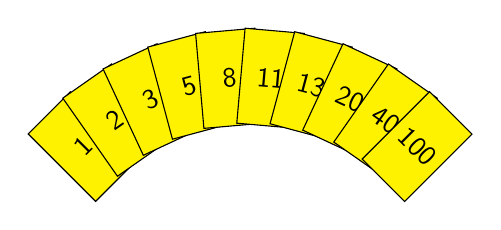
\begin{tikzpicture}
        \tikzset{every node/.style={font=\sffamily}}
        \foreach [count=\i] \ii in {1,2,3,5,8,11,13,20,40,100} {
            \pgfmathsetmacro{\ang}{145-\i*10}
            \pgfmathsetmacro{\rot}{45-((\i-1)*10)}
            \node[minimum width = 5ex, minimum height=8ex, rotate around={\rot:(0,0)}, draw, fill=yellow] at (\ang:3) {\ii};
        }
    \end{tikzpicture}
\end{document}